\newcommand{\wvec}{\begin{pmatrix}1 \\ 0 \end{pmatrix}}
\newcommand{\svec}{{\begin{pmatrix}0 \\ 1 \end{pmatrix}}}
\newcommand{\kalpha}{\ket{\alpha}}
\newcommand{\kbeta}{\ket{\beta}}
\newcommand{\kpsi}{\ket{\psi}}




\newpage
\thispagestyle{empty}
\chapter{Preliminaries}\label{chapter one}
In this chapter we present the basic theoretical knowledge necessary to understand this thesis. We begin by introducing graph theory, random walks and quantum walks. We then discuss the quantum search problem firstly introduced by Grover and the quantum walks implementation for the unstructured search by Childs and Goldstone. Then we present the adiabatic theorem and its application to the adiabatic quantum search, studying the global and local adiabatic evolution. Lastly we look at the differences between the quantum walks approach and the local adiabatic evolution search by Roland and Cerf, which sets the basis from which our work is carried on.

\section{Introduction to graph theory}\label{sec:introduction to graph theory}
A graph G is defined as a ordered pair $(V,E)$, where V is a set of vertices and E is a set of edges, that represents the connection between any two pair of vertices. A vertex is usually indicated by the coursive letter $v$, and the corresponding edge connecting $v$ to $w$ is given by $(v,w)$. \\

\noindent
A graph can be characterized by many properties. Throughout our work we will only consider \textit{simple graphs} characterized by being \textit{undirected}, namely the edges $E$ are symmetric, having no self loops such that $(v,v)\notin G$ and having no multiple equivalent edges. Additionally we require the graph to be \textit{connected}, i.e. each vertex can be reached by any other following a path through the available edges.

\noindent
We then define the \textit{vertex degree} $d_j$, that represents, given a vertex $j$, the number of edges that are incident to the vertex $j$\footnote{For an undirected graph the degree does not dependend on the edges incident from or to the selected vertex, while generally this is not true}. \\

\noindent
If indeed any two vertices $i$ and $j$ are connected by an edge $(i,j)$ we define them as \textit{adjacent}, and from this we can construct an analytical representation of a graph, given by an N-dimensional square matrix called \textit{adjacency matrix}, usually referred as A. The adjacency matrix is defined as following \footnote{If we had to define the adjacency matrix for an unspecified graph the value of $A_{ij}$ is not necessarily equal to one, but a general $a_{ij}$ since it takes into account the possibilities of self loops and multiple equivalent edges. For the simple graphs consider in this thesis the given definition suffices.}:
\begin{equation}
A_{ij} = \begin{cases} 1 & \mbox{if }(i,j)\in G \\ 0 & \mbox{otherwise} \end{cases}
\end{equation}
which represents the connectivity of the graph. \\
Furthermore, we can introduce a diagonal matrix $D$ that encodes the informations of the vertex degrees for a particular graph $G$. Calling the N vertices of the graph as $j=1,2..N$ the matrix D is defined as:
\begin{equation}
    D = diag(d_1,..., d_N)
\end{equation}
where $d_j$ is the degree of the vertex $j$.
In this particular context a natural operative basis arises, in which one can associate to each ordered vertex of the graph a vector of the standard basis of the N-dimensional vector space. \\ \\


In order to study the dynamics of the system we introduce the \textit{Laplacian matrix L}, also known as the \textit{discrete Laplacian operator}. It is defined as
\begin{equation}
    L = D-A
\end{equation}
where $D$ is the diagonal degrees matrix and $A$ is the adjacenty matrix. The discrete Laplacian operator is the analog of the continous Laplace operator on discrete domain, and for the finite, undirected, simple and connected graphs can charactarized by the following properties:
\begin{itemize}
  \item $L$ is symmetric given that both $D$ and $A$ are symmetric
  \item the sum of all elements over a row/column equals to zero
  \item has a null eigenvalue which corresponds to the eigenvector $\ket{\Psi_0} = \frac{1}{\sqrt{N}}\big(1,1,...,1\big)$
\end{itemize}
As previously mentioned we can associate every vertex to a basis vector of the N-dimensional vector space. Similarly we can expand this notation to an N-dimensional Hilbert space, where we can use the following Dirac notation to describe the vertex. This formalism allows us to write the Laplacian matrix in convenient quantum mechanical form using the projectors $\ket{j}\bra{i}$
\begin{equation}
  \ket{1}=\begin{bmatrix} 1 \\ 0 \\ \vdots \\ 0\end{bmatrix}, \hspace{15pt}\ket{2}=\begin{bmatrix}0\\1\\\vdots\\0\end{bmatrix}, \hspace{15pt}\ket{N}=\begin{bmatrix}0\\0\\\vdots\\N\end{bmatrix}
\end{equation}


In the following paragraphs we give a brief description of the graphs that will be consider throughout the work. \\

    \subsection{Cycle graph}\label{subsec:cycle graph}
    %\addcontentsline{toc}{subsection}{Cycle Graph}
        A N-dimensional cycle graph $Cy(N)$ is a monodimensional structure with periodic boundary conditions $\ket{N+1}=\ket{N}$. The Laplacian is given by
        \begin{equation}
            L = 2\sum_{k=1}^{N}\ket{k}\bra{k} - \sum_{k=1}^{N-1}\ket{k}\bra{k+1} - \sum_{k=2}^{N}\ket{k}\bra{k-1}- \ket{N}\bra{1}-\ket{1}\bra{N}
        \end{equation}
        A pictorial representation of a cycle graph is given in Fig with the corrisponding laplacian matrix.
        \begin{figure}[ht]
          \centering
          \begin{tabular}{ccc}
            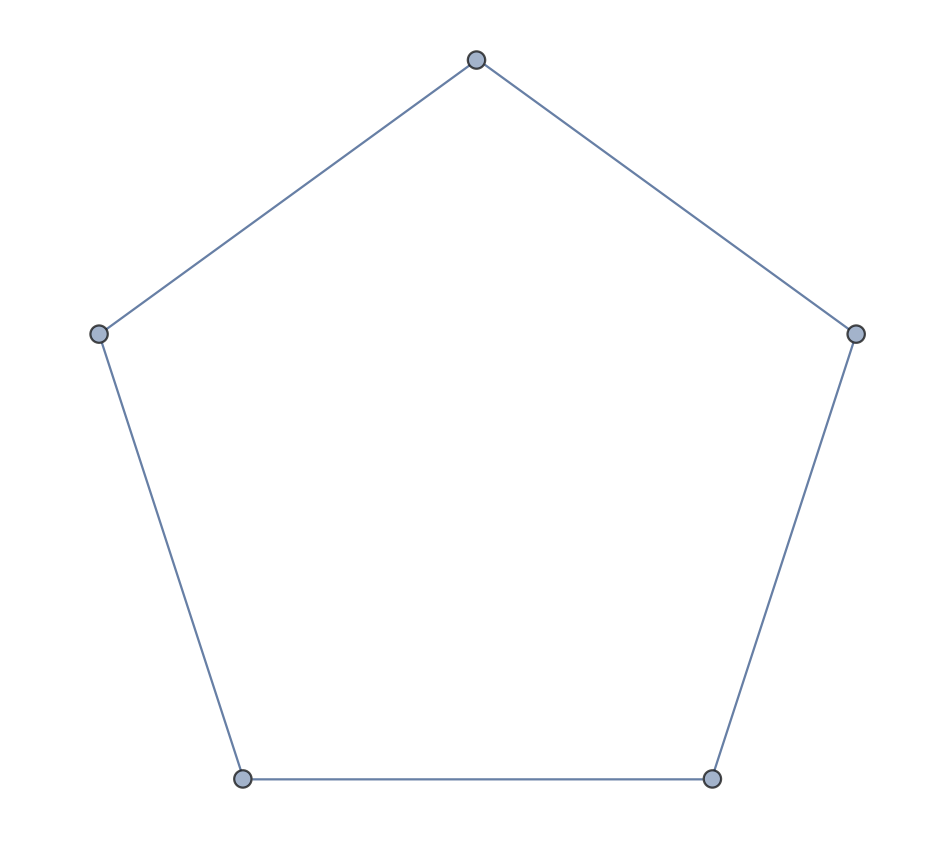
\includegraphics[width=55mm]{./figures/chapter1/cycle} & \hspace{20pt} &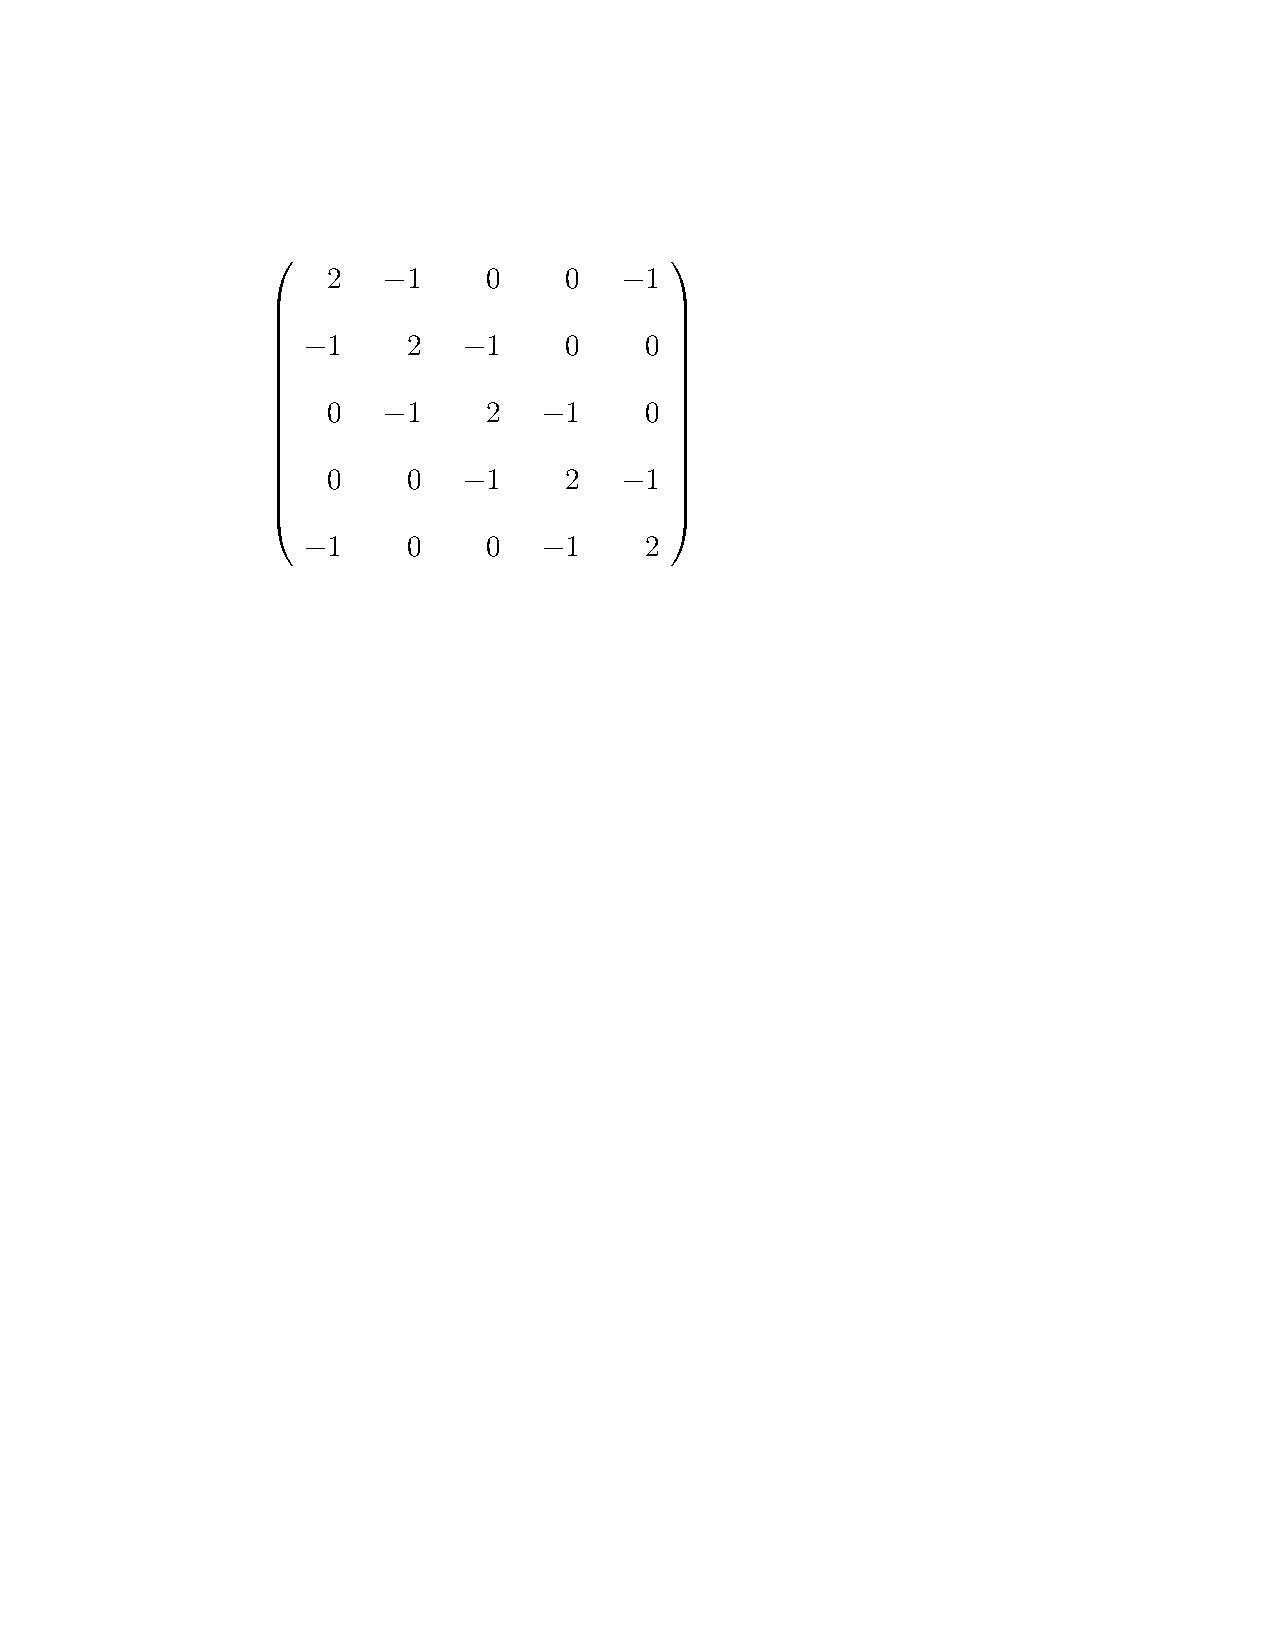
\includegraphics[width=50mm]{./figures/chapter1/Laplacian} \\[0.5cm]
          (a)  & & (b) \\[6pt]
          \end{tabular}
          \caption[Pictorial representation of a cycle graph, and matricial representation for the Laplacian]{Pictorial representation of a cycle graph with 5 nodes (a), and the matricial representation for the Laplacian of Cy(5)}
        \end{figure}
    \vspace{-0.7cm}
    \subsection{Complete graph}\label{subsec:complete graph}
    %\addcontentsline{toc}{subsection}{Complete Graph}
        A graph with N vertices is said to be complete if every node is adjacent to all the other N-1 nodes, thus representing a finite bidimensional structure. Its Laplacian matrix is given by:
        \begin{equation}
            L = (N-1)\sum_{j=1}^{N}\ket{j}\bra{j} - \sum_{k\neq j}\ket{j}\bra{k}
        \end{equation}
        A pictorial representation of a complete graph is given in figure. We will refer to this type of graph with $C(N)$.
        \begin{figure}[hb]
          \centering
          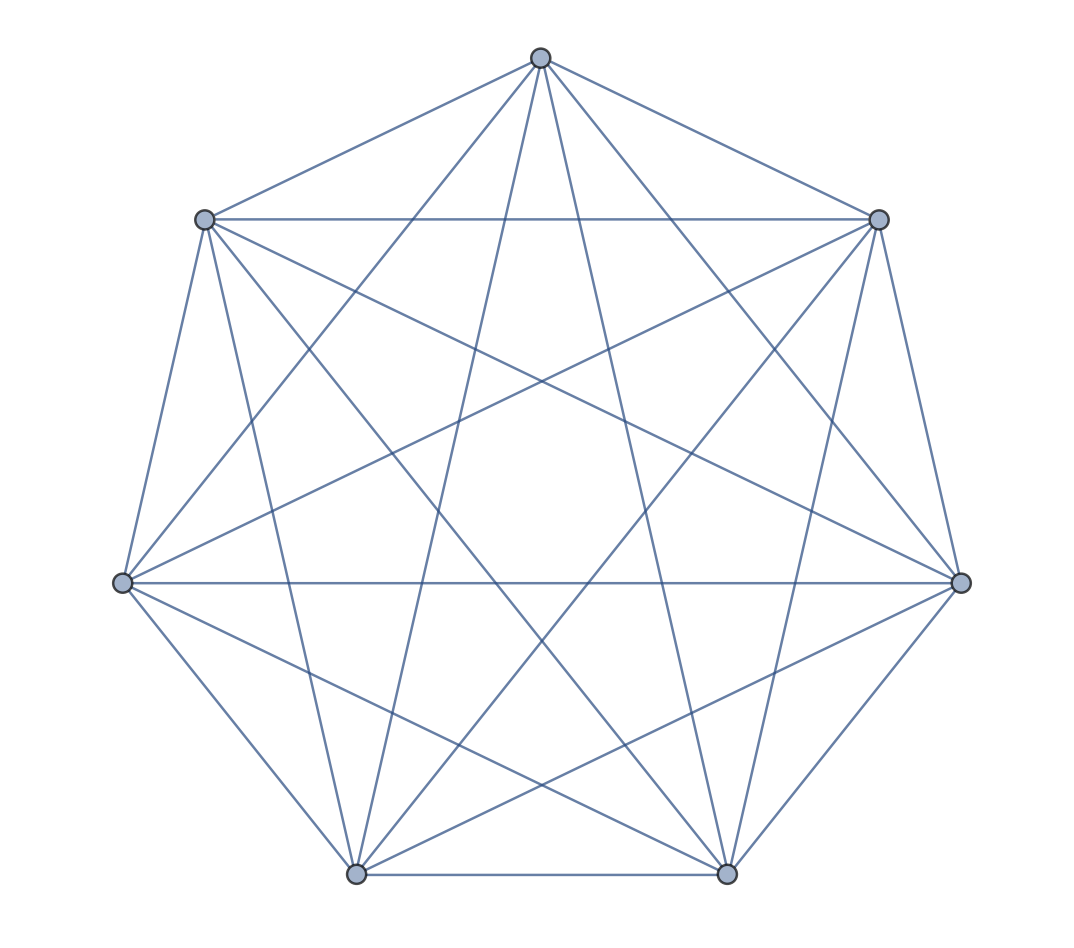
\includegraphics[width=50mm]{./figures/chapter1/complete}
          \caption[Pictorial representation of a complete graph]{Pictorial representation of a complete graph with N=7}
        \end{figure}

\section{Quantum walks}\label{sec:quantum walks}
The continous time quantum walk (CTQW) is the direct analogue of the classical continous time random walk (CTRW). We begin by considering the classical one, expanding later on the quantum mechanical counterpart. \nocite{Mulken2011} \\

A continous-time random walk is a stochastic process by which a walker randomly moves on a particular mathematical structure, which in our scenario is a graph $G$.
Let $j$ be a note of a graph $G$ and the initial node, such date the initial state of the system is $\ket{j}$\footnote{With abuse of notation we represent both the classical and the quantum mechanical vertex with the Dirac notation $\ket{j}$}. Then, we denote the transition probability of the walker to go from node j to a node k in a time t with $p_{k,j}(t)$. The state after time $t$ is given by $\ket{j;t}$, such that the overlap with node $k$ is $\braket{k|j;t}=p_{j,k}(t)$. \\
The dynamics resulting in the state $\ket{j;t}$ follows from transition rates per unit time between two nodes. In particular these transition rates are the components of the so-called \textit{transfer matrix} $T$, namely $T_{ij}= \bra{k}T\ket{j}$ . If we assume a Markovian process, the following master equation defines the CTRW evolution:
\begin{equation}
  \frac{d}{dt}p_{k,j}(t) = \sum_{l}T_{kl}p_{l,j}(t)
  \label{rw_master}
\end{equation}
In the simplest case, where the transitions rates for all edges are equal, the transfer matrix is closely related to the Laplacian matrix through :
\begin{equation}
  T = -\gamma L
\end{equation}
where $\gamma$ is the transition rate. The solution of \cref{rw_master}, along with the normalization constrains $\sum_{k=1}^{N}p_{k,j}(t) = 1 \hspace{3pt} \forall t$, is given by
\begin{equation}
  p_{ij}(t)= \braket{k|e^{Tt}|j} = \braket{k|e^{-\gamma At}|j}
\end{equation}
Turning to quantum mechanics the evolution of any physical system obeys the Schroedinger equation, and QWs represent no exception. The dynamics of the CTQW is governed by a specific Hamiltonian $H$, such that the Schroedinger equation for the transition \textit{amplitudes} $\alpha_{i,j}(t)$ is given by
\begin{equation}
  \frac{d}{dt}\alpha_{i,j}(t) = -i \sum_{l}H_{k,l}\alpha_{l,j}(t)
\end{equation}
where $H$ is the Hamiltonian of the systemm, and for semplicity we assume $\hbar = 1$. The formal solution of such differential equation is given by
\begin{equation}
  \alpha_{l,j}(t) = \braket{k|e^{-iHt}|j}
  \label{qw_master}
\end{equation}
where $e^{-iHt}$ is the quantum mechanical time-evolution operator. We immediately notice the similar structure of equations (\ref{rw_master}) and (\ref{qw_master}), with the only difference - apart from the imaginary unit - that the first is a differential equation for transition probabilities while the latter allows to compute transition amplitudes. The similarity is further pushed by Farhi and Gutmann, proposing to identify the Hamiltonian $H$ of the system with the negative of the classical transfer matrix $T$ \cite{Childs2001}, which as we've seen previously is the Laplacian of the graph \footnote{Please note that in this particular scenario the transition amplitude $\gamma$ is set to one, and assumed to be equal for all vertex transition.}:
\begin{equation}
  H = -T = L
  \label{qw_Hamiltonian}
\end{equation}
Therefore the Laplacian matrix completely determines the evolution of the quantum system as well as the classical scenario.



\section{Grover's quantum search}\label{sec:grover search}
In 1997 Lov K. Grover addressed the search problem through a quantum mechanical algorithm \cite{Grover1997}. The search problem itself can be formulated in the following way: given an unsorted database containing N items, with only one satisfing a given condition, that one item has to be retrieved. Once an item is examined, it's possible to determine whether it represents the solution or not in just one step.
Classically, the most efficient algorithm has to check each and every item in the database individually. If the item checked satisfies the condition the process stops, otherwise it will continue to examine the remaining items until the solution is find. On average, the algorithm will have to check $N/2$ items before finding the desired one.\\On the other hand, Grover's quantum mechanical approach takes advantage of the \textit{superposition} of states in a quantum system, and by having the input and output in such superposition can find the desired item in $O(\sqrt{N})$ \textit{quantum mechanical steps}, instead of $O(N)$ classical steps. As we shall see later, this quantum mechanicals steps consists of an elementary unitary operation. \\

\noindent
Let's look at the algorithm to the quantum search problem more in detail, in particular setting the stage for the search algorithm in terms of an \textit{oracle}, which plays a central role in Grover's search and throughout our work. Additionally, this allows us to present a very general description of the search procedure, and a geometric way to visualize its action \cite{Nielsen2000}. \\

\noindent
Suppose we want to search through a search space of $N$ elements, and let's consider the indices of such elements - instead of the actual elements - that are numbers from 0 to $N-1$. In order to easily store the index in $n$ bits we consider $N=2^n$, and assume that the particular search problem has only one solution. We can now easily represent one instance of the search, i.e. checking if the item satisfies a particular condition, with a function $f(x)$, where $x$ is the index integer ranging from 0 to $N-1$. The function is such that if $x$ represents the solution to the search problem $f(x)=1$, and $f(x)=0$ if not a solution. In particular we suppose that we are supplied by a quantum \textit{oracle} $O$ with the ability to \textit{recognize} the solution of the search problem. The action of the oracle $O$ is to \textit{mark} the solution by applying a phase, namely $\ket{x}\xrightarrow{O}(-1)^{f(x)}\ket{x}$. \\ In a simplified manner, the quantum search algorithm proposed by Grover consists of reapeted application of a quantum subroutine known as the \textit{Grover iteration} or \textit{Grover operator} $G$ defined as:
\begin{equation}
  G = (2\ket{\psi}\bra{\psi}-I)O
\end{equation}
Where $\psi$ is the initial state.
The questions that arises is what does this Grover operator do. We can show that it can be regarded as a \textit{rotation} in the 2-dimensional space spanned by the beginning vector $\ket{\psi}$ and the vector $\ket{w}$ representing the solution to the search problem. We can then define the normalized state $\ket{\alpha}$ and $\ket{\beta}$:
\begin{equation}
    \ket{\alpha} = \frac{1}{\sqrt{N-1}}\sum_{x\neq w}\ket{x}
\end{equation}
\vspace{-0.5cm}
\begin{equation}
  \ket{\beta} = \ket{w}
\end{equation}
representing respectively, the superposition of all states that are not a solution and the state of the solution. Therefore the initial state $\ket{\psi}$ can be re-expressed by:
\begin{equation}
  \ket{\psi}= \sqrt{\frac{N-1}{N}}\ket{\alpha} + \sqrt{\frac{1}{N}}\ket{\beta}
\end{equation}
The effect of $G$ can be understood by realizing that the oracle $O$ performs a \textit{reflection} of $\kpsi$ about the vector $\kalpha$ in the plane defined by $\kalpha$ and $\kbeta$. Then, $2\kpsi\bra{\psi}-I$ performs another reflection about the vector $\kpsi$. As can be seen in figure?, the product of these two reflections i a rotation. By applying the grover operator $k$ times we can rotate the initial state vector $\kpsi$ close to $\kbeta$, that is, the solution to the search problem. The number of iterations necessary - for which the derivation is not of our interest in the scope of this thesis - is given by $\frac{\pi}{4}\sqrt{N}$.
\begin{figure}[ht]
  \centering
  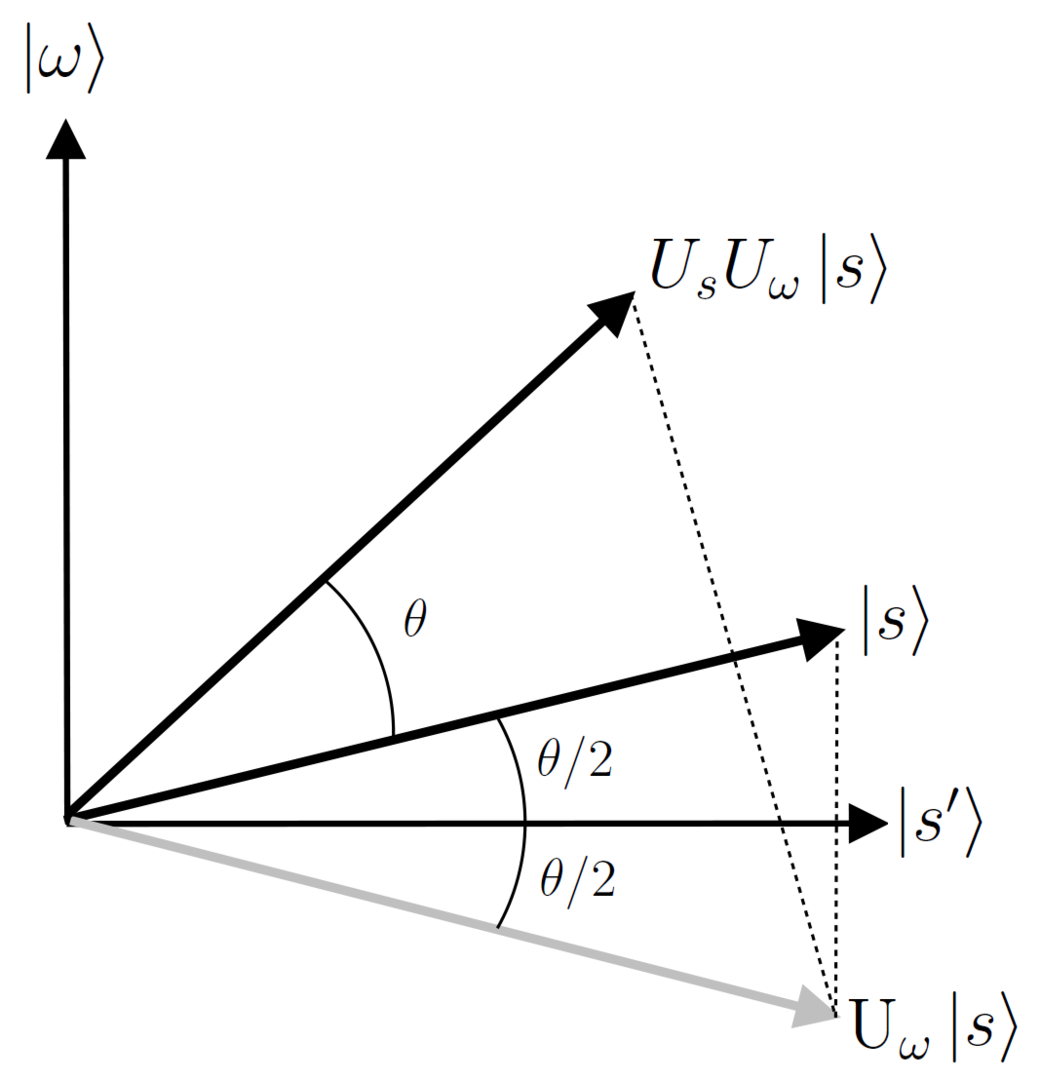
\includegraphics[width=70mm]{figures/chapter1/grover_reflection}
  \caption[Action of the Grover operator]{\textbf{Action of the Grover operator }$\bm{G}$: The figure shows the action of the Grover operator $G=(2\kpsi\bra{\psi} -I)O$. Starting from the initial state $\kpsi$ the action of the Oracle $O$ reflects it about the vector $\kalpha$. Then, the action of $(2\kpsi\bra{\psi}-I)$ is an additional reflection about $\kpsi$. The application of the Grover operator for $\pi/4\sqrt{N}$ times rotates the inital state bringing it close to $\kbeta$, that is, the solution of the search problem.}
  \label{fig:grover_operator}
\end{figure}


\noindent
To summarize, G is the rotation in the 2-dimensional space spanned by $\kalpha$ and $\kbeta$. Repeated application of the Grover operator rotate the initial state vector $\kpsi$ close to $\kbeta$. For applications of $G$ in the order of $O(\sqrt{N})$, a measurement of the state in the computational basis produces with high probability $\kbeta$ as the outcome, that is, the solution to the search problem.


\section{Search by quantum walks}\label{sec:search quantum walk}
The search problem first introduced by Grover can be reformulated in terms of search based on a continous-time quantum walk on a graph \cite{Childs2004}. \\In order to do so we need to modify the quantum walk Hamiltonian of \cref{qw_Hamiltonian} so that the vertex $\ket{w}$ is somewhat special. Therefore, an \textit{oracle Hamiltonian} is introduced:
\begin{equation}
  H_w = -|w\rangle\langle w|
\end{equation}
that has energy zero for all but the vertex $|w\rangle$ for which it has energy $-1$. Therefore the Grover problem becomes finding the ground state of this Hamiltonian. \\To implement the search we consider the Hamiltonian
\begin{equation}
  H = \gamma L + H_w = \gamma L -|w\rangle\langle w|
\end{equation}
where L is the laplacian of the graph $G$, that as we've seen in section? governs the evolution of the quantum walk.\\
The quantum search works as following:
\begin{itemize}
  \item we consider the balanced superposition of all possible states, namely
  \begin{equation}
    |s\rangle = \frac{1}{\sqrt{N}}\sum_j|j\rangle
  \end{equation}

  \item we run the quantum walk for a time $T$ and find the corrisponding evolved state using the Hamiltonian $H$
  \begin{equation}
  |\psi(T)\rangle = U(T)|s\rangle  = \mbox{exp}\Big\{-\frac{i}{\hbar}HT\Big\}|s\rangle
  \end{equation}
  (Note that this evolution is valid only for time-independent Hamiltonians.)

  \item we then measure the occupation probability of the targer
  \begin{equation}
    p = |\langle w|\psi(T)\rangle|^2
  \end{equation}

\end{itemize}
\noindent
The objective is to find the optimal value of $\gamma$ so that the success probability $|\braket{w|\psi(T)}|^2$ is as close as possible to 1 for the smallest $T$. \\
It is interesting to notice that the oracle introduced in this fashion is exactly the continous-time version of the reflection $R_w$ in Grover's algorithm \cite{Wong2016} because by itself it only evolves the marked vertex $\ket{w}$ by a phase
\begin{equation}
  e^{-i\ket{w}\bra{w}t}\ket{w} = e^{-it}\ket{w}
\end{equation}
while leaving the other vertices unchanced, thus making this the continous-time version of a yes/no oracle. \\


\noindent
We can turn our attention on trying to understand why we should expect this algorithm to give a success probability for some values of $\gamma, T$. To motivate this we need to frame the problem in terms of Hamiltonian spectrum \cite{Childs2004}. In particular we look at the two extremes, namely $\gamma\rightarrow\infty$ and $\gamma\rightarrow 0$.
\begin{itemize}
  \item as $\gamma\rightarrow\infty$ the contribution of $H_w$ is somewhat negligible, to the point that the ground state of $H$ is $\ket{s}$\footnote{Note that regardless of the graph topology considered, $\ket{s}$ is the ground state of the Laplacian, with $L\ket{s} = 0$.}
  \item on the other hand, if $\gamma\rightarrow 0$ the contribution of the Laplacian to the overall Hamiltonian $H$ disappears and thus the ground state of $H$ is close to $\ket{w}$
\end{itemize}
We expect that for some intermediate $\gamma$ the ground state will transition from $\ket{w}$ to $\ket{s}$ and thus could have substantial overlap on both for a certain value of $\gamma$. Additionally, if the first excited states have substantial overlap at such values of $\gamma$, then the Hamiltonian will drive transitions between two states, thus rotating the state from $\ket{s}$ to one with substantial overlap with $\ket{w}$, giving the success probability that we previously talked about. In particular this transition will happen in a time that dependes on the Hamiltonian eigenvalues separation between the first and ground state, namely $1/(E_1-E_0)$.

%This is a good description of the algorithm if the dimension of the graph is sufficiently high.  However, if we consider a $d$-dimensional lattice with $d$ independent of $N$ we still see that for a critical value of $\gamma$ the state switches from the ground state to the first excited state, but for $d<4$ the $\ket{w}$ state does not have substantial overlap on the ground and fist excited state, thus the algorithm does not work. \\

\subsection{Search on the complete graph}\label{subsec:search qw complete graph}
We now look at the complete graph which can be thought of having dimension proportional to N and represents the simples example of the quantum walk search application \cite{Childs2004}. \\We begin by noticing that adding a multiple of the identity matrix to the Laplacian only contributes a global unobservable phase. We add $-NI$ so that:
\begin{equation}
  L - NI = N\ket{s}\bra{s}
\end{equation}
This gives us the following Hamiltonian:
\begin{equation}
  H = -\gamma N \ket{s}\bra{s} - \ket{w}\bra{w}
\end{equation}
In particular we know that this Hamiltonian acts non-trivially in a two dimensional subspace spanned by $\ket{s}$ and $\ket{w}$, thus making it stright-forward to compute its spectrum. If we use the $\{\ket{w}, \ket{r}\}$ basis, the Hamiltonian can be expressed in the following way:
\begin{equation}
  H = \frac{-1}{N} \begin{pmatrix} N+1 & \sqrt{N-1}\\ \sqrt{N-1} & N-1 \end{pmatrix}
\end{equation}
Applying the time-evolution operator to the initial state $\ket{s}$, the system at time $t$ will be
\begin{equation}
  \ket{\psi(t)} = e^{it}
  \begin{pmatrix}
  \frac{1}{\sqrt{N}}\cos(\frac{t}{\sqrt{N}}) +i\sin(\frac{t}{\sqrt{N}})\\
  \sqrt{\frac{N-1}{N}}\cos(\frac{t}{\sqrt{N}})
  \end{pmatrix}
  \label{eq:qw_state}
\end{equation}
and for $t=\pi\sqrt{N}/2$ the system reaches a success probability of 1, namely
\begin{equation}
  p = \Big|\braket{w|\psi(t)}\Big|^2_{t=\pi\sqrt{N}/2} = 1
\end{equation}
Thus the walk rotates the state from $\ket{s}$ to $\ket{w}$ in $O(\sqrt{N})$.

\section{Search by adiabatic evolution}\label{sec:adiabatic evolution}
We now address the computation by adiabatic evolution firstly introduced by Farhi et al., that takes advantage of the adiabatic theorem to find the solution of a computational problem \cite{Farhi2000}. We begin by looking at the \textit{adiabatic theorem} and its implication. Then, an overview of the adiabatic implementation of the algorithm for solving the unstructured search problem is given which has a time scaling of $O(N)$. Lastly, we see how applying the adiabatic theorem \textit{locally} can lead to a time of order $O(\sqrt{N})$ which is optimal.

    \subsection{Adiabatic theorem}\label{subsec:adiabatic theorem}
    A quantum system evolves according to the Schroedinger equation
    \begin{equation}
        i\frac{d}{dt}|\psi(t)\rangle = H(t)|\psi(t)\rangle
    \end{equation}
    and defining the instantaneous eigenstates and eigenvalues of H(t) by
    \begin{equation}
        H\ket{\psi_l(t)} = E_l\ket{\psi_l(t)}
    \end{equation}
    such that $E_0(t) \leq E_1(t) \leq ... \leq E_{N-1}(t)$. \\
    The adiabatic theorem states that if the gap between the two lowest energy levels, $E_{1}(t) - E_{0}(t) > 0$, is stritcly greater than zero then for $T\rightarrow \infty$ the probability of being in the ground state is equal to one, namely
    \begin{equation}
        \lim_{T \to \infty} \braket{\psi_0(T)|\psi(T)}= 1
    \end{equation}
    This means that if the system is chosen to evolve at a slow enough rate, the instantaneous Hamiltonian will remain in the ground state throughout the evolution. Furthermore it's convenient to parametrize the Hamiltonian as $H(s)$, where $s=t/T$, with $t \in [0,T]$ so that $s \in [0,1]$.
    Let's now define the energy minimum gap between the lowest eigenvalues of $H$ by
    \begin{equation}
        g_{min} = \min_{0 \leq s \leq 1} (E_1(s)-E_0(s))
    \end{equation}
    This allows to find a minimum time $T^*$ such that, for $T\gg T^*$ the probability of being in the ground state $\ket{\psi_0}$ is arbitrarily close to 1. In details, $T^*$ is given by:
    \begin{equation}
        T^* = \frac{\varepsilon}{g^{2}_{min}}
        \label{eq:adiabatic_time}
    \end{equation}
    where
    \begin{equation}
        \varepsilon = \max_{0 \leq s \leq 1} \Big| \Big\langle \psi_1(s)\Big| \frac{dH(s)}{d} \Big| \psi_0(s)\Big\rangle\Big|
    \end{equation}\\


\noindent
Let's now discuss how to take advantage of the adiabatic theorem. It is often presented a problem Hamiltonian $H_P$ whose ground state is not so straight forward to find; on the other hand we can prepare the system in a beginning Hamiltonian $H_B$ whose ground state is known. The problem Hamiltonian encodes the solution of the problem, while the beginning Hamiltonian is a tool for easily preparing the state to be evolved. The adiabatic evolution then consists, assuming that the ground state of $H_P$ is unique, in having a time dependent Hamiltonian $H(s)$ that interpolates between $H_B$ and $H_P$
    \begin{equation}
        H(s) = (1-s)H_B + s H_P
    \end{equation}
    In this way we can prepare for $s=0$ the system in $H_B$ and let it evolve so that for $s=1$ it reaches $H_P$. Therefore, if the system is made to evolve sufficiently slowly we will find ourself in the ground state of the problem Hamiltonian, that is exactly the solution.

    \subsection{Global adiabatic evolution}\label{subsec:global adiabatic}
    Let's now apply what just seen to the unsorted search problem \cite{Roland2002}. As done in \Cref{sec:grover search} we consider an unsorted database of $N$ elements such that $N=2^n$, so that the elements in this particular basis can be written as $\ket{i}$, with $i=0,...,N-1$. The marked state can be then denoted as $\ket{w}$, and we begin by considering the initial state as the superposition of all the elements $\ket{i}$:
    \begin{equation}
      \ket{\psi_0}=\frac{1}{\sqrt{N}}\sum_{i=1}^{N-1}\ket{i}
    \end{equation}
    With this in mind we design two particular Hamiltonians $H_0$ and $H_w$ such that $\ket{\psi_0}$ is the ground state of the first while $\ket{w}$ is the ground state of the latter:
    \begin{equation}
      H_0 = I- \ket{\psi_0}\bra{\psi_0}
      \label{eq:adiabatic_ground}
    \end{equation}
    \vspace{-1cm}
    \begin{equation}
      H_w = I- \ket{w}\bra{w}
      \label{eq:adiabatic_first}
    \end{equation}
    The time-dependent Hamiltonian follows from the adiabatic implementation discussed in \Cref{sec:adiabatic evolution}, where $H_0$ is the beginning Hamiltonian and $H_w$ is the problem Hamiltonian. It thus consists in a linear interpolation between $H_0$ and $H_w$:
    \begin{equation}
      H(t) = (1-s)H_0 + sH_w
    \end{equation}
    where $s=t/T$ is the linear interpolating schedule.\\ \\
    The search routine runs as usual, beginning with preparing the system in the state $\ket{\psi(0)}=\ket{\psi_0}$ and then applying the Hamiltonian $H(t)$ for a time $T$. we are interested in finding the time-dependent condition such that the system evolves sufficiently slowly, allowing us to find the solution $\ket{w}$ with high probability. First, we determine the quantity $\braket{\frac{dH}{dt}}$:
    \begin{equation}
      \braket{\frac{dH}{dt}}_{0,1} = \frac{ds}{dt}\braket{\frac{dH}{ds}}_{0,1} = \frac{1}{T}\braket{\frac{dH}{ds}}_{0,1}
    \end{equation}
    We then find the eigenvalues of the Hamiltonian and determine the separation $g$ between the ground state and first excited one, namely $E_1$ and $E_0$, as a function of the interpolating schedule $s$:
    \begin{equation}
      g=\sqrt{1-4\frac{N-1}{N}s(1-s)}
      \label{separation}
    \end{equation}
    we are interested in the minimum gap $g_{\min}$ which is found for $s=1/2$. Additionally we find that $\big|\braket{\frac{dH}{ds}}_{0,1}\big| \leq 1$, therefore \Cref{eq:adiabatic_time} becomes:
    \begin{equation}
      \frac{\big|\braket{\frac{dH}{ds}}_{0,1}\big|}{g_{\min}^2} \leq \varepsilon
      \label{adiabatic_condition}
    \end{equation}
    so that the adiabatic condition is verified, and thus the Hamiltonian stays in the ground state at all times, provided that :
    \begin{equation}
      T\geq N/\varepsilon
      \label{eq:adiabatic_scaling_global}
    \end{equation}
    Therefore the computation time is of order $N$, showing no speed up compared to the classical search.

    \subsection{Local adiabatic evolution}\label{subsec:local adiabatic}
    Roland and Cerf showed that the adiabatic evolution can be improved by applying the adiabatic condition of \cref{adiabatic_condition} locally instead of globally \cite{Roland2002}. If we look at the plot of the separation $g$ we see that the adiabatic condition is critical only for $s=1/2$ where it reaches its minimum.
    \begin{figure}[h]
      \centering
      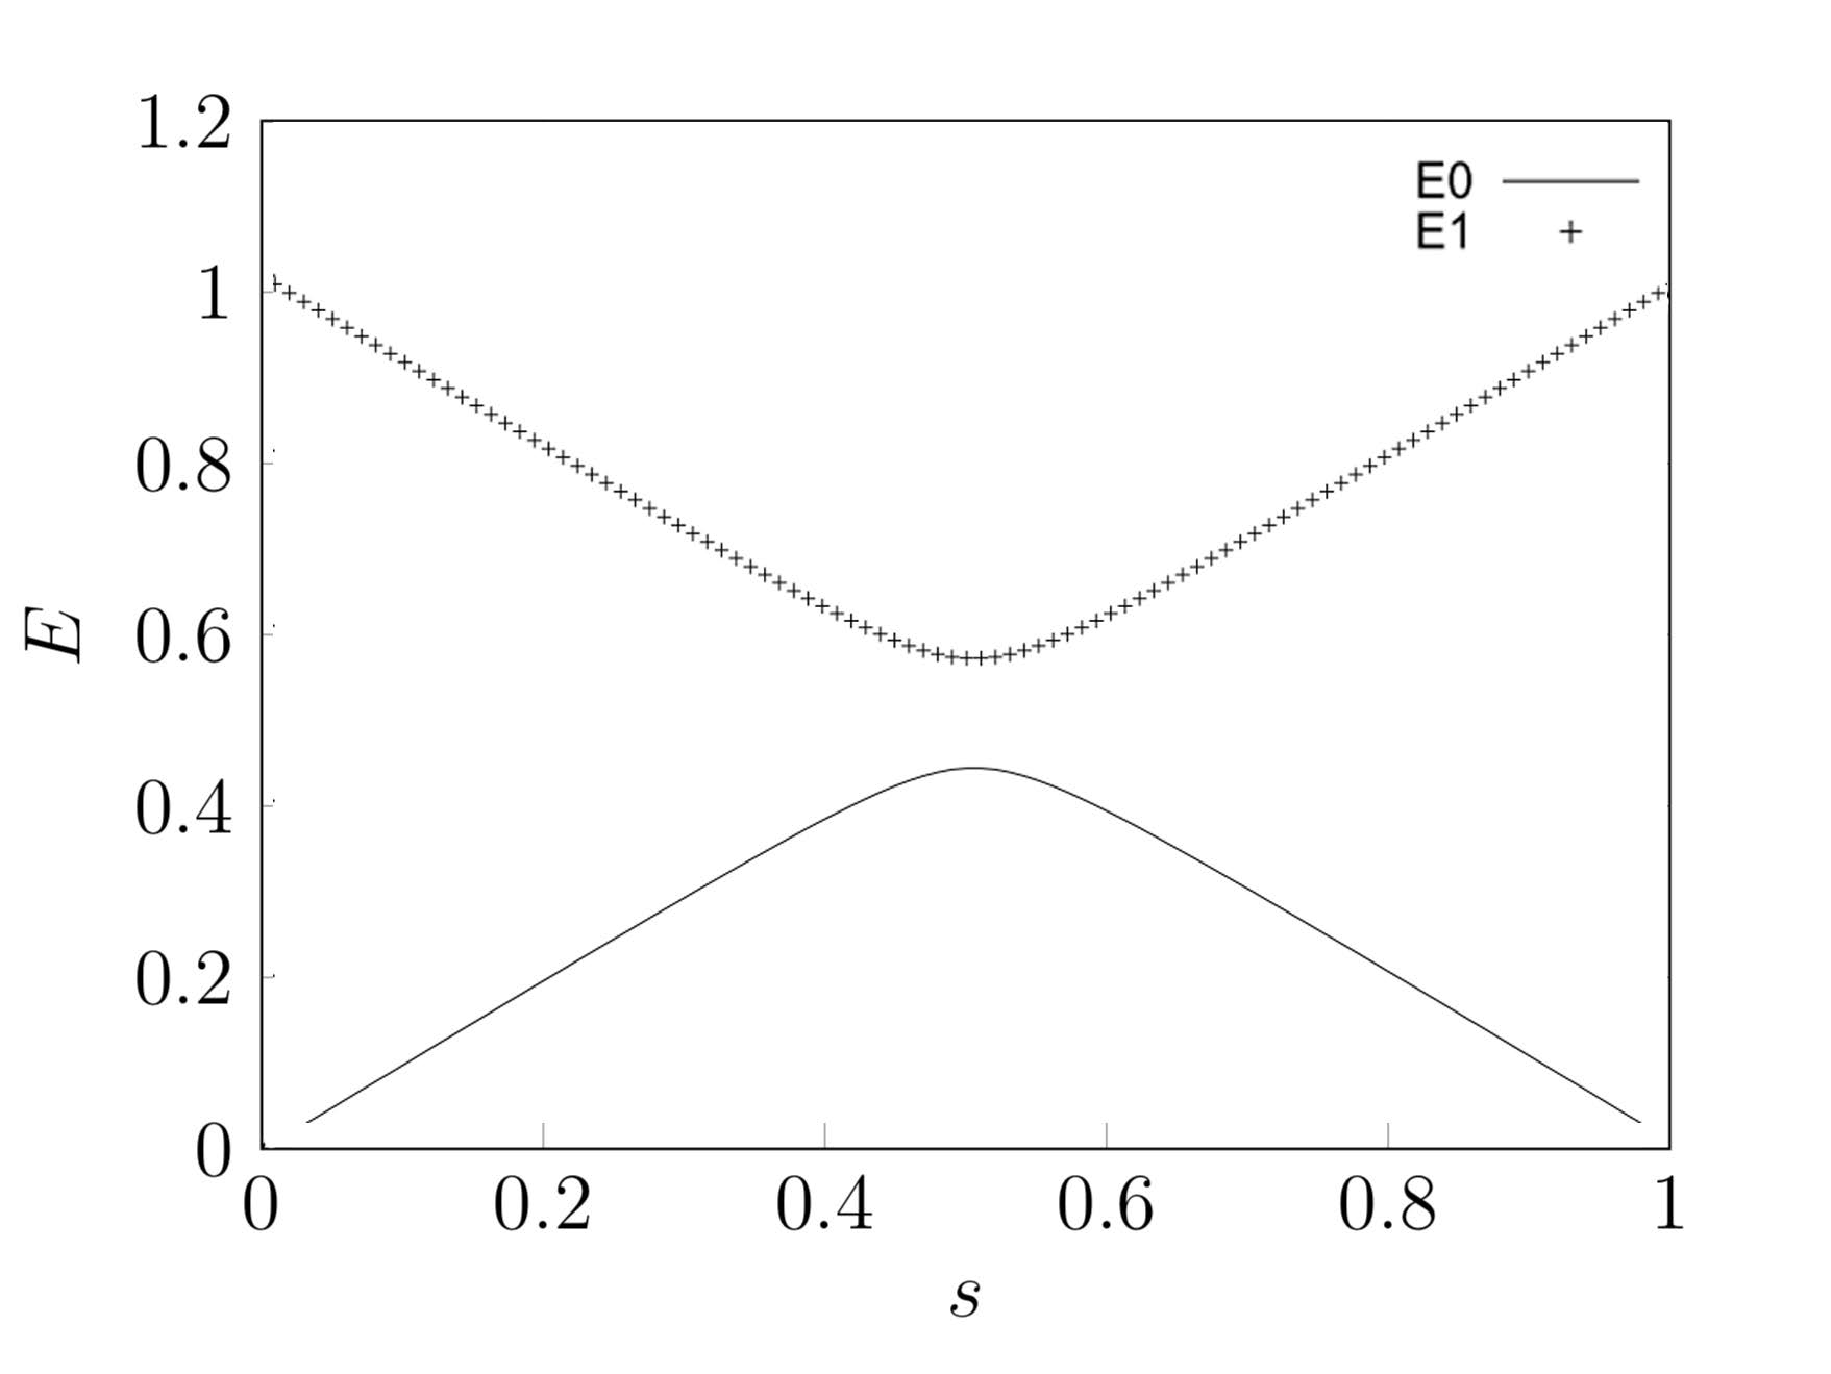
\includegraphics[width=80mm]{figures/chapter1/separation}
      \caption[Eigenvalue separation of the time-dependent Hamiltonian $H(s)$ as a function of the reduced time $s$, for N=64]{Eigenvalue separation of the time-dependent Hamiltonian $H(s)$ as a function of the reduced time $s$, for N=64. \textit{Figure from Roland and Cerf} \cite{Roland2002}}
      \label{separation_figure}
    \end{figure}
    At the beginning and at the end of the evolution the separation is large enough so that the adiabatic condition and thus the time necessary for the system to evolve adiabatically is small, allowing for better time scaling. The improvement comes in the form of the interpolating schedule, following the idea that it should be steeper for large separation $g$ and flatter for small separation around $s=1/2$. Let's see how can this be done. \\ \\
    We divide the interval $[0,T]$ into infinitesimal intervals $dt$ and adapt the evolution rate $\frac{ds}{dt}$ to the local adabatic condition. In this way we can find the optimal $s(t)$, with boundary conditions $s(0)=0$ and $s(T)=1$. We find the new adiabatic condition for all time $t$:
    \begin{equation}
      \Big|\frac{ds}{dt}\Big|\leq\varepsilon\frac{g^2(t)}{\big|\braket{\frac{dH}{ds}}_{0,1}\big|}
    \end{equation}
    Using \cref{separation} and $\big|\braket{\frac{dH}{ds}}_{0,1}\big| \leq 1$ and Hamiltonian is chosen to evolve with the interpolating schedule that is solution of the following differential equation (with $\varepsilon<<1$):
    \begin{equation}
      \frac{ds}{dt} = \varepsilon g^2(t) = \varepsilon\Big[1-4\frac{N-1}{N}s(1-s)\Big]
    \end{equation}
    After integration we get the following
    \begin{equation}
      t =\frac{1}{2\varepsilon}\frac{N}{\sqrt{N-1}}\Big[\arctan\big(\sqrt{N-1}(2s-1)\big) + \arctan{\sqrt{N-1}}\Big]
    \end{equation}
    By inverting we find the interpolating schedule $s(t)$ as can be seen in \cref{interpolating_schedule}. In order to determine the computation time of this algorithm. To do so we evaluate $s=1$ and in the approximation that $N>>1$ we get:
    \begin{equation}
      T = \frac{\pi}{2\varepsilon}\sqrt{N}
    \end{equation}
    which represents a great improvement on \Cref{eq:adiabatic_scaling_global} Indeed we have a quadratic speed up compared to the global adiabatic evolution, and thus this algorithm can be seen as the adiabatic implementation of the Grover's search algorithm.
    \begin{figure}[h]
      \centering
      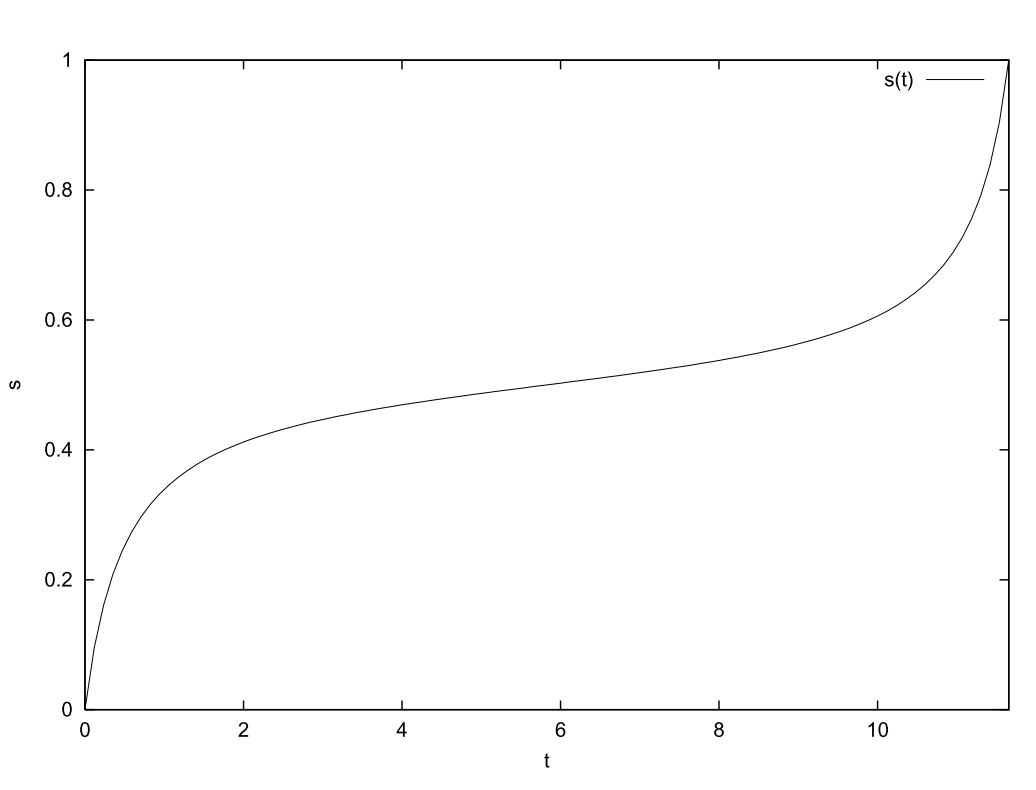
\includegraphics[width=80mm]{figures/chapter1/interpolating_schedule}
      \caption[Roland and Cerf interpolating schedule for the unstructured search with N=64]{Roland and Cerf interpolating schedule for the unstructured search with N=64. \textit{Figure from Roland and Cerf} \cite{Roland2002}}
      \label{interpolating_schedule}
    \end{figure}



\section{Impossibility of a search algoritm based on adiabatic quantum walks}\label{impossibility}
In this section we show that an \textit{adiabatic quantum walks} (AQW) based search algorithm cannot be implemented with the usual Grover's oracle and requires a more sophisticated structure. This section, based on a paper by Wong et al. \cite{Wong2016}, sets the basis on which our work builds upon. \\ \\
In the previous sections we discussed Grover's original discrete-time search algorithm (GR), Farhi and Gutmann's quantum walk analogue (FG) and Roland and Cerf's adiabatic analogue (RC). Throught the discussion we analysized the systems in a 2-dimensional subspace spanned by $\big\{\ket{w}, \ket{r}\big\}$.This allows to visualize the evolution of the quantum algorithm on the two dimensional Bloch sphere and compare the path taken by each different approach. In particular we notice that the original Grover's algorithm and the Roland and Cerf's local adiabatic evolution follow the same path on the $xz$-plane since they both always have real coefficients, as can be seen in \Cref{fig:blochsphere_Grover,fig:blochsphere_RC} respectively. On the other hand the quantum walk formulation of Farhi and Gutmann has an unmeasurable complex phase thus it evolves on a different path on the $yz$-plane, see \Cref{fig:blochsphere_FG}.
\begin{figure}[h]
     \centering
     \subfloat[Grover]{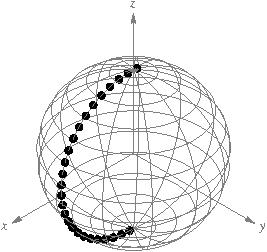
\includegraphics{figures/chapter1/blochsphere_Grover}\label{fig:blochsphere_Grover}}
     \subfloat[Roland-Cerf]{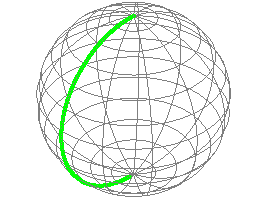
\includegraphics{figures/chapter1/blochsphere_RC}\label{fig:blochsphere_RC}}
     \subfloat[Farhi-Gutmann]{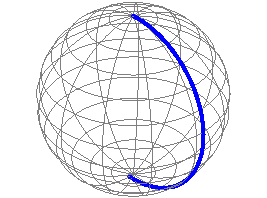
\includegraphics{figures/chapter1/blochsphere_FG}\label{fig:blochsphere_FG}}
     \caption[Evolution of the quantum algorithms on the bloch sphere]{\textbf{Evolution of the quantum algorithms on the bloch sphere}. The figure shows the evolution of quantum algorithm on the Bloch sphere with marked vertex $\ket{w}$ at the North Pole and the equal superposition of the unmarked vertices $\ket{r}$ at the South Pole, and $N=1024$: (a) Grover's original discrete-time search algorithm, (b) Roland and Cerf's local adiabatic evolution analogue and (c) Farhi and Gutmann's quantum walk analogue. \textit{Wong et al. (2016)} \cite{Wong2016}}
     \label{fig:blochsphere}
\end{figure}

\noindent
This substantial difference of the path taked by the different algorithms is exacly what Wong et al. investigate, in particular with the goal of determine which adiabatic algorithm does follow the same path of the quantum walk algorithm of Farhi and Gutmann in order to implement an adiabatic quantum walk based search algorithm. \\

\noindent
To do so they constructed an Hamiltonian starting from the following states, with the first represents the ground state and the latter the first (and only) excited state - rememeber that the Grover's search rotates the initial state over the final state, thus the first excited state is the orthogonal of the ground state.
\begin{equation}
  \ket{\psi_0(t)} = \alpha(t)\ket{w} + \beta(t)\ket{r}
\end{equation}
\vspace{-0.5cm}
\begin{equation}
  \ket{\psi_1(t)} = \beta(t)\ket{w} - \alpha^*(t)\ket{r}
\end{equation}
where the coefficients are given by the components of $\ket{\psi_0(t)}$ of \cref{eq:qw_state}\footnote{Note that the global phase $e^{it}$ is dropped.}.
The Hamiltonian is then given by the linear combination of $\ket{\psi_0(t)}$ and $\ket{\psi_1(t)}$:
\begin{equation}
  H(t) = \lambda_0\ket{\psi_0}\bra{\psi_0} + \lambda_1\ket{\psi_1}\bra{\psi_1}
\end{equation}
which allows to determine the final time-dependent \textit{adiabatic} Hamiltonian - where the time-dependence is given by the interpolating schedule $s(t)$:
\begin{equation}
  H(s) = \sqrt[4]{\frac{s(1-s)}{4\varepsilon^2N}}\Big[ (1-s)H_0 + sH_f + \sqrt{s(1-s)}H_e\Big]
\end{equation}
where the interpolating schedule is given by $s(t)=\sin^2\big(\frac{t}{\sqrt{N}}\big)$. Indeed the system evolves from $t=0$ to $t=\frac{\pi}{2}\sqrt{N}$ as we would expect. Looking closely the Hamiltonian $H_0$ is the beginning Hamiltonian, $H_f$ is the final Hamiltonian - encoding the solution of the search problem - and $H_e$ is an \textit{extra} Hamiltonian, a common tecnique for manupulating the evolution of the path of adiabatic algorithms\footnote{The extra Hamiltonian commonly appears as $s(s-1)$, while the one considered in this scenario is given by the square root of such value \cite{Wong2016}.}. Let's now look at the consequences of this Hamiltonian, looking at $H_0$, $H_f$ and $H_e$ individually. \\
$H_0$ has ground state $\ket{s}$ and excited state $\ket{s^\perp}$ with respective eigenvalues $-1$ and $+1$, thus the Hamiltonian can be written as:
\begin{equation}
  H_0  = \ket{s^\perp}\bra{s^\perp} - \ket{s}\bra{s}
\end{equation}
Similarly, the final Hamiltonian $H_f$ has ground state $\ket{w}$ and excited state $\ket{r}$ with eigenvalues $+1$ and $-1$:
\begin{equation}
  H_f =  \ket{r}\bra{r} - \ket{w}\bra{w}
\end{equation}
It's immediate to notice that these two Hamiltonian look fairly similar to the initial and final Hamiltonian of the standard adiabatic quantum search algorithm of \Cref{eq:adiabatic_ground,eq:adiabatic_first}. Although the similarities look at first sight promising, the extra Hamiltonian $H_e$ and the interpolating schedule $s(t)$ change completely the evolution of the system. In particular, if we look at the Hamiltonian $H_e$ - given by:
\begin{equation}
  H_e = 2i\sqrt{\frac{N-1}{N}}\big(\ket{r}\bra{w} - \ket{w}\bra{r}\big)
\end{equation}
we see that rather than having the standard yes/no oracle given by $\ket{w}\bra{w}$, this extra Hamiltonian introduces a more powerful structure, driving the evolution between $\ket{w}$ and $\ket{r}$ insted of just applying a phase to the targer state $\ket{w}$ like in the standard Grover's algorithm. This is a confirmation that the oracle is no more the usual Grover's yes/no oracle, and althought this a proof that an adiabatic evolution following the quantum walk path does exists it abandons the usual notion of the oracle and does not solve the search problem itself as originally posed by Grover. \\

\noindent
The difference between the Quantum Walks and the Adiabatic Evolution approach is not a measure of the performance of the algorithms, since both, individually, solve the Grover's problem in $O(\sqrt{N})$ time, but illustrate that the ``\textit{how} they compute is different, even though \textit{what} they compute is the same '' \cite{Wong2016}.\\

\noindent
Althought the worke by Wong et al. showed that is not possible to implement an adiabatic quantum walk algorithm that solves the search problem, it leaves space to a time-dependent algorithm \textit{inspired} by the adiabatic evolution but that it's free from the constrains of the adiabatic condition. From this last considerations we develop our thesis. In the next chapter we summarize the work done and gives some interesting insights and properties of the quantum walks search algorithm with time-dependent Hamiltonians.


%%%
%TIME DEPENDENT: HEATMAP PLOT FOR DIFFERENT INTERPOLATING SCHEDULES
%%

\begin{figure}[ht]
  \centering
  \subfloat[][$s_L(t)$]
  {
    \begin{tikzpicture}
      \begin{axis}[name=plot,
      zmin=0,zmax=1,
      view={0}{90},
      colormap={inferno}{rgb255=(248,251,155) rgb255=(251,179,21) rgb255=(236,103,38) rgb255=(187,54,84) rgb255=(119,29,109) rgb255=(49,9,92) rgb255=(1,1,8)},
      colorbar,
      colorbar right,
      point meta min=0,
      point meta max=0.25,
      width = 60mm,
      height= 60mm,
      xlabel = $\bm{T}$,
      ylabel = $\bm{\gamma}$
      ]
      \addplot3 [surf] table[x=a,y=b,z=c]{./Data/fig5/fig5_51_lin.txt};
      \end{axis}
    \end{tikzpicture}
  }
  \subfloat[][$s_S(t)$]
  {
    \begin{tikzpicture}
      \begin{axis}[name=plot,
      zmin=0,zmax=1,
      view={0}{90},
      colormap={inferno}{rgb255=(248,251,155) rgb255=(251,179,21) rgb255=(236,103,38) rgb255=(187,54,84) rgb255=(119,29,109) rgb255=(49,9,92) rgb255=(1,1,8)},
      colorbar,
      colorbar right,
      point meta min=0,
      point meta max=0.25,
      width = 60mm,
      height= 60mm,
      xlabel = $\bm{T}$,
      ylabel = $\bm{\gamma}$
      ]
      \addplot3 [surf] table[x=a,y=b,z=c]{./Data/fig5/fig5_51_sqrt.txt};
      \end{axis}
    \end{tikzpicture}
  }
  \qquad
  \subfloat[][$s_C(t)$]
  {
    \begin{tikzpicture}
      \begin{axis}[name=plot,
      zmin=0,zmax=1,
      view={0}{90},
      colormap={inferno}{rgb255=(248,251,155) rgb255=(251,179,21) rgb255=(236,103,38) rgb255=(187,54,84) rgb255=(119,29,109) rgb255=(49,9,92) rgb255=(1,1,8)},
      colorbar,
      colorbar right,
      point meta min=0,
      point meta max=0.25,
      width = 60mm,
      height= 60mm,
      xlabel = $\bm{T}$,
      ylabel = $\bm{\gamma}$
      ]
      \addplot3 [surf] table[x=a,y=b,z=c]{./Data/fig5/fig5_51_cbrt.txt};
      \end{axis}
    \end{tikzpicture}
  }
  \subfloat[][$s_{NL}(t)$]
  {
    \begin{tikzpicture}
      \begin{axis}[name=plot,
      zmin=0,zmax=1,
      view={0}{90},
      colormap={inferno}{rgb255=(248,251,155) rgb255=(251,179,21) rgb255=(236,103,38) rgb255=(187,54,84) rgb255=(119,29,109) rgb255=(49,9,92) rgb255=(1,1,8)},
      colorbar,
      colorbar right,
      point meta min=0,
      point meta max=0.25,
      %colorbar style={
      %at={(0.75,-0.8)},
      %anchor=center,
      %},
      width = 60mm,
      height= 60mm,
      xlabel = $\bm{T}$,
      ylabel = $\bm{\gamma}$
      ]
      \addplot3 [surf] table[x=a,y=b,z=c]{./Data/fig5/fig5_51_cerf.txt};
      \end{axis}
    \end{tikzpicture}
  }



  \caption{\textbf{Probability heatmap plot for the time-dependent Hamiltonian, for different shapes of s(t) and \bm{$Cy(51)$}.} The figure shows the probability heatmap plots for a circular graph of $N=51$ evaluated using the time-dependent Hamiltonian using the following interpolating schedules: (a) linear, (b) $s_S(t)$, (c) $s_C(t)$ and (d) non-linear $s_{NL}(t)$.}
  \label{fig:heatmap_time_dependent}
\end{figure}

